\documentclass{article}
\usepackage{amsmath}
\usepackage{graphicx}
\usepackage[utf8]{inputenc}
\usepackage{parskip}
\usepackage[symbol]{footmisc}

\newtheorem{theorem}{Theorem}[section]
\renewcommand{\thefootnote}{\fnsymbol{footnote}}

\setcounter{secnumdepth}{0}

\date{}
\author{Kaan Aksoy | March 12, 2020}

\begin{document}

\maketitle
\section{Random Quadratic Equations}

\subsection{Problem}

What is the probability that the following quadratic 
equation has real roots?
$$x^2 + 2bx + c =0$$

\subsection{Solution}

We begin by applying the quadratic formula to the 
equation given above:

$$x = \frac{-2b \pm \sqrt{4b^2-4c}}{2}$$

Rearranging the contents of $\sqrt{4b^2-4c}$ shows that 
the roots are real if and only if the following holds:

$$4b^2-4c > 0$$
$$c < b^2$$

\begin{figure}[h]
\centering
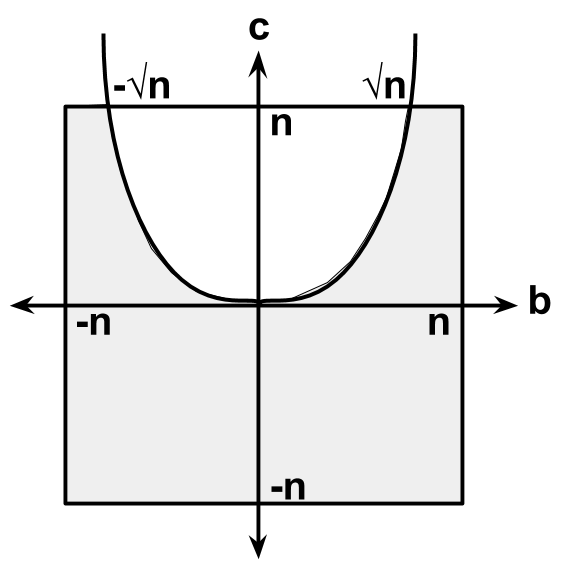
\includegraphics[width=4cm]{Problem50_RandomQuadraticEquation.png}
\caption{The shaded area represents equations with real roots}
\end{figure}


We can calculate the probability that $c < b^2$ geometrically. 
We begin by drawing a $2n$ by $2n$ square centered at the origin. 
The graph of $c=b^2$ intersects the square at $b=\pm \sqrt{n}$. 
Within the square, the shaded region below the parabola 
represents equations with real roots. 

To find the probability of real roots, $P$, we can calculate the  
proportion of the shaded area with respect to the entire square. 
We will consider the limiting value of this proportion as $n$ tends 
towards $\infty$:

\begin{equation*}
\begin{split}
P &= \lim_{n \to \infty} \frac{4n^2 - \int_{-\sqrt{n}}^{\sqrt{n}}n-b^2db}{4n^2} \\
&= \lim_{n \to \infty} \frac{4n^2 - \frac{4}{3}n^{\frac{3}{2}}}{4n^2} \\
&= \lim_{n \to \infty} 1 - \frac{3}{\sqrt{n}} \\
&= 1
\end{split}
\end{equation*}

Thus, the probability of the equation having real roots is $1$.
\end{document}